\section{Progress}

\begin{frame}{Overall Design}
    \begin{figure}[!htb]
        \centering
        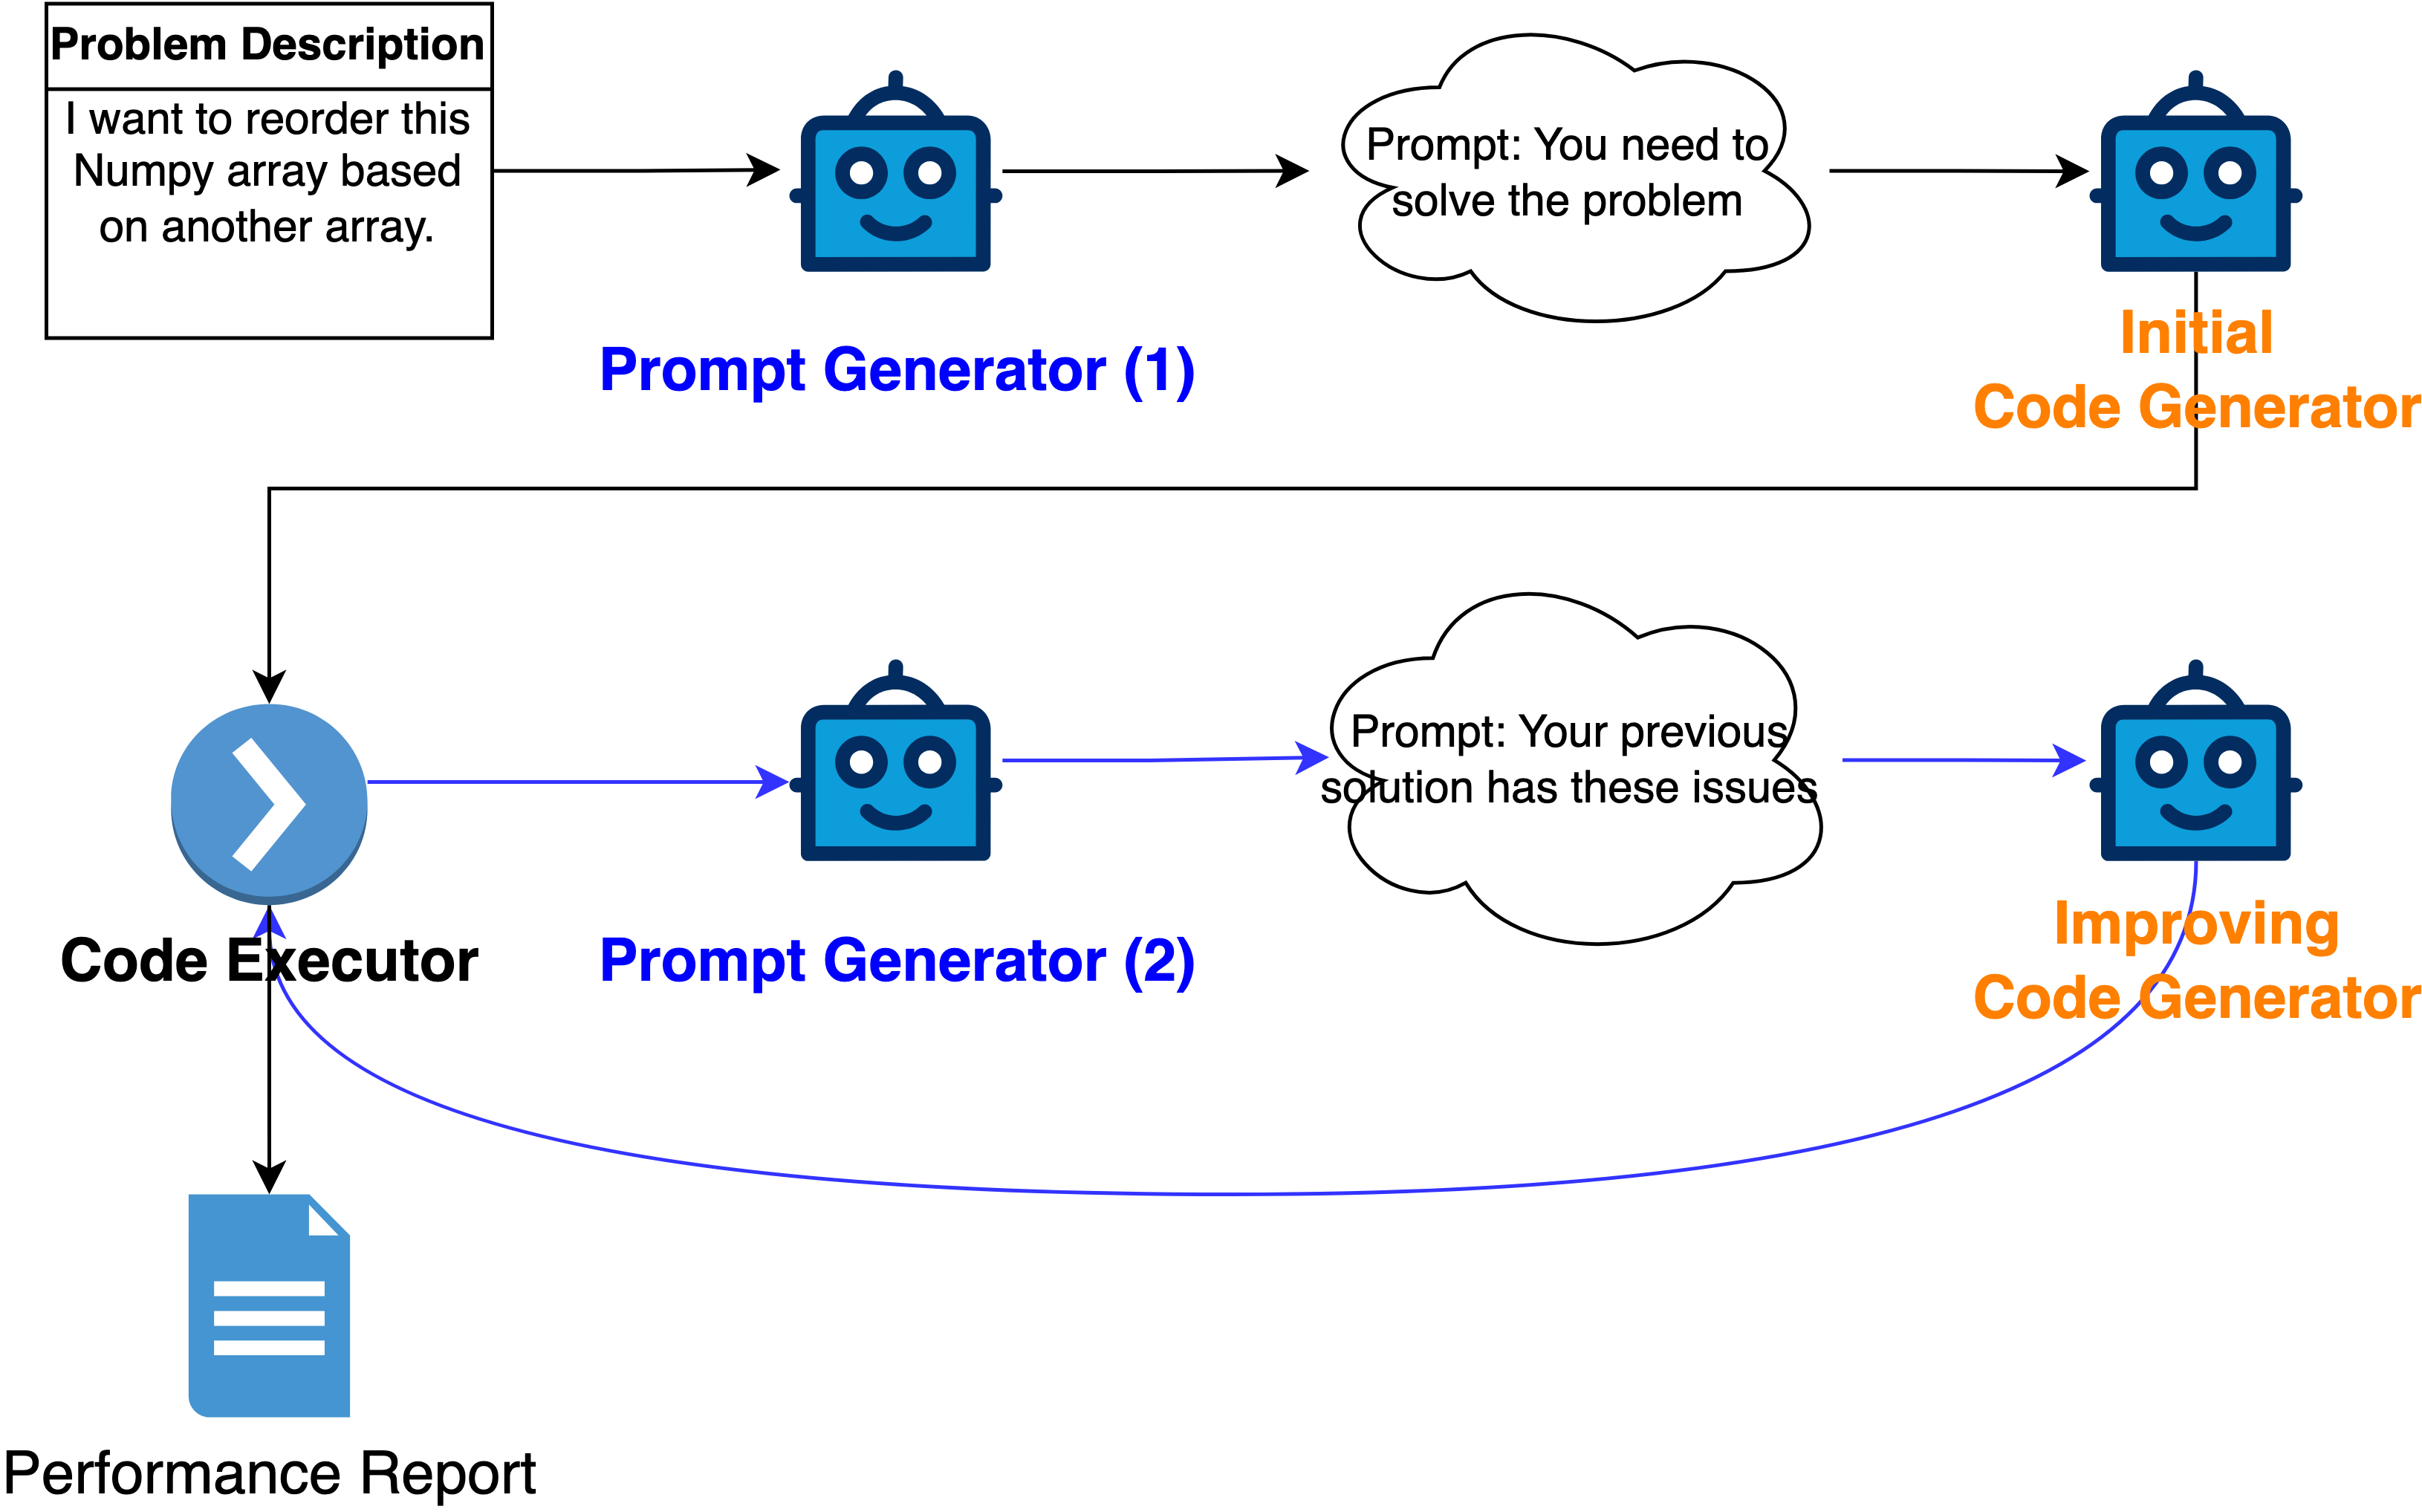
\includegraphics[width=0.9\textwidth]{img/selfdebug_design}
        \captionsetup{font=small,labelformat=empty}
        \caption{The modules of the proposed system.}
    \end{figure}
\end{frame}

\begin{frame}{Progress Update \: 08 Mar 2024}
    Completed:
    \begin{itemize}
        \item Prompt Generator (1) with Zero-shot prompts (baseline)
        \item Initial-Code Generator with ChatGPT 3.5 API
        \item Code Executor on Virtual environment to run test cases
        \item Performance Report using accuracy score
    \end{itemize}

    Baseline Results:
    \begin{tabular}{lr}
        Library    & Accuracy \\
        \hline
        Matplotlib & 18.06\%  \\
        Scipy      & 16.04\%  \\
        Pandas     & 8.93\%   \\
        Numpy      & 5.91\%   \\
        Sklearn    & 9.57\%   \\
        Tensorflow & 17.78\%  \\
        Pytorch    & 2.94\%   \\
    \end{tabular}
\end{frame}

\begin{frame}{Progress Update \: 08 Mar 2024}
    Next Steps:
    \begin{itemize}
        \item Prompt Generator (2) with CoT prompts based on code execution feedback
        \item Correcting-Code Generator
    \end{itemize}
\end{frame}

\begin{frame}{Progress Update \: 29 Mar 2024}
    Completed:
    \begin{itemize}
        \item Prompt Generator (1) with CoT prompts
        \item Prompt Generator (2) with direct feedback from code execution
        \item Correcting-Code Generator
    \end{itemize}

    Improved Results:
    \begin{tabular}{lr}
        Library    & Accuracy \\
        \hline
        Matplotlib & 41.94\%  \\
        Scipy      & 16.98\%  \\
        Pandas     & 23.71\%  \\
        Numpy      & 15.91\%  \\
        Sklearn    & 41.74\%  \\
        Tensorflow & 28.89\%  \\
        Pytorch    & 38.24\%  \\
    \end{tabular}
\end{frame}

\begin{frame}{Progress Update \: 29 Mar 2024}
    Example of CoT prompt:

    Here are some step-by-step suggestions to help solve the problem:

    1. \textbf{Suggestion 1}: First, let's understand the problem. The goal is to shuffle the order of the DataFrame's rows according to a given list. The list represents the desired order of the rows.

    2. \textbf{Suggestion 2}: To achieve this, we can use the `iloc' function in pandas to select the rows of the DataFrame based on the given list. The `iloc' function allows us to select rows by their integer position.

    3. \textbf{Suggestion 3}: Start by creating a new DataFrame that contains the shuffled rows. You can do this by using the `iloc' function with the given list as the index. For example, `shuffled\_df = df.iloc[List]`.

    4. \textbf{Suggestion 4}: Finally, assign the shuffled DataFrame to the `result' variable. This will be the solution to the problem. For example, `result = shuffled\_df`.
\end{frame}

\begin{frame}{Progress Update \: 29 Mar 2024}
    Next Steps:
    \begin{itemize}
        \item Analyze the failed test cases to improve the Prompt Generator (2)
        \item Connect with more LLMs: Claude 2.0, GPT-4, etc.
    \end{itemize}
\end{frame}

\begin{frame}{Progress Update \: 8 Apr 2024}
    Completed:
    \begin{itemize}
        \item Improve Prompt Generator (2)
        \item Use ChatGPT 4 API for Correcting-Code Generator
    \end{itemize}

    Improved Results:
    \begin{tabular}{lr}
        Library    & Accuracy \\
        \hline
        Matplotlib & 72.90\%  \\
        Scipy      & 44.34\%  \\
        Pandas     & 77.66\%  \\
        Numpy      & 63.64\%  \\
        Sklearn    & 80.87\%  \\
        Tensorflow & 71.11\%  \\
        Pytorch    & 73.53\%  \\
    \end{tabular}
\end{frame}
